\section{Příklad 4}
% Jako parametr zadejte skupinu (A-H)
\ctvrtyZadani{C}

Při použití metody smyčkových proudů je využito druhého Kirchhoffova zákona, který říká, že \textit{součet úbytků napětí na~spotřebičích se v~uzavřené části obvodu, smyčce, rovná součtu napětí zdrojů v~této smyčce}. Při jejím výpočtu hledáme hodnoty fiktivních proudů, které obíhají uvnitř jednotlivých elementárních smyček. Pro každou smyčku pak sestavíme rovnici podle druhého Kirchhoffova zákona, přičemž jednotlivá napětí vyjádříme pomocí zavedeného fiktivního proudu smyčky. Ze soustavy těchto rovnic zjistíme fiktivní smyčkové proudy, pomocí kterých vypočítáme napětí na jednotlivých spotřebičích.

Obvod ze zadání rozdělíme na tři smyčky $\color{red}A$, $\color{red}B$, $\color{red}C$, jak je naznačeno na obrázku \ref{fig:circ-4-1}. Orientace smyček je zvolena zcela náhodně.
\begin{figure}[ht]
    \centering
    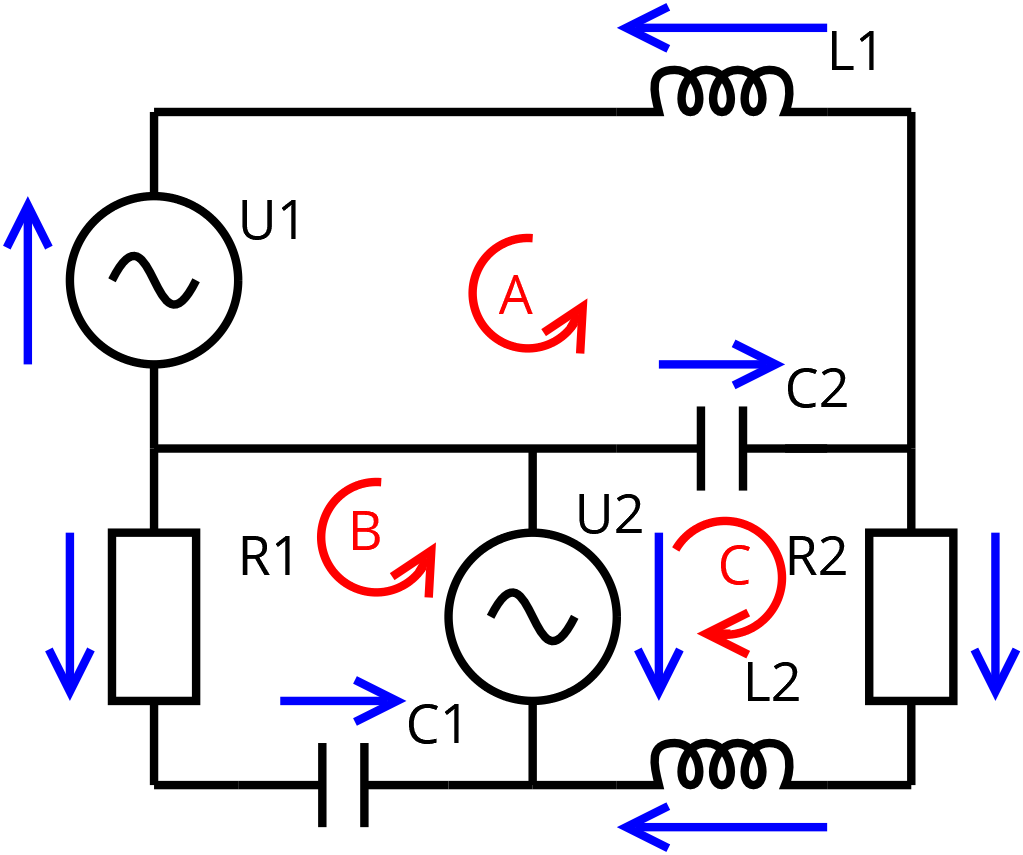
\includegraphics[width=7cm]{diagrams/Diagram12.png}
    \caption{Obvod se zaznačenými smyčkami a směry napětí ve speciálním časovém okamžiku $t = \frac{\pi}{2\omega}$.}
    \label{fig:circ-4-1}
\end{figure}
Předpokládejme, že smyčkou $\color{red}A$ prochází proud $I_A$, podobně ve~zbylých dvou smyčkách. Pro jednotlivé smyčky můžeme zapsat rovnice podle druhého Kirchhoffova zákona:
\begin{align*}
    \textcolor{red}{A}\!:\  & U_{C_2} + U_{L_1} - U_1 = 0 \\
    & (I_C + I_A) Z_{C_2} + I_A Z_{L_1} - U_1 = 0 \\
    & (Z_{L_1}+Z_{C_2}) I_A + Z_{C_2} I_C = U_1 \\
    \\
    \textcolor{red}{B}\!:\  & U_{R_1} + U_{C_1} - U_2 = 0 \\
    & I_B Z_{R_1} + I_B Z_{C_1} - U_2 = 0 \\
    & (Z_{R_1} + Z_{C_1}) I_B = U_2 \\
    \\
    \textcolor{red}{C}\!:\  & U_{R_2} + U_{L_2} - U_2 + U_{C_2} = 0 \\
    & I_C Z_{R_2} + I_C Z_{L_2} - U_2 + (I_C + I_A) Z_{C_2} = 0 \\
    & Z_{C_2} I_A + (Z_{R_2} + Z_{C_2} + Z_{L_2}) I_C = U_2 
\end{align*}
Vzniklé rovnice pak můžeme zapsat do matice s proměnnými $I_A$, $I_B$, $I_C$:
\[
\begin{pmatrix}[ccc|c]
    Z_{L_1} + Z_{C_2} &                 0 & Z_{C_2}                     & U_1 \\
    0                 & Z_{C_1} + Z_{R_1} &                           0 & U_2 \\
    Z_{C_2}           &                 0 & Z_{R_2} + Z_{C_2} + Z_{L_2} & U_2
\end{pmatrix}
\]

Nyní vypočítáme úhlovou frekvenci a impedance jednotlivých komponent, ty pak dosadíme do~zjištěné matice:
\begin{gather*}
    \omega = 2 \pi f = 150 \pi \\
    Z_{R_1} = R_1 = \SI{10}{\ohm} \\
    Z_{R_2} = R_2 = \SI{13}{\ohm} \\
    Z_{L_1} = j \omega L_1 = 33\pi j \\
    Z_{L_2} = j \omega L_2 = \frac{21}{2}\pi j \\
    Z_{C_1} = -\frac{j}{\omega C_1} = -\frac{2000}{69\pi} j \approx \num{-9.2264}j \\
    Z_{C_2} = -\frac{j}{\omega C_2} = -\frac{4000}{51\pi} j \approx \num{-24.9655}j \\
    \\
    \everymath{\displaystyle}
    A = \begin{pmatrix}[ccc|c]
    \left(33\pi-\frac{4000}{51\pi}\right) j & 0 & -\frac{4000}{51\pi} j & 35 \\
    0 & 10 -\frac{2000}{69\pi} j &                           0 & 45 \\
    -\frac{4000}{51\pi} j & 0 & 13 - \left(\frac{4000}{51\pi} + \frac{21}{2}\pi\right) j & 45
    \end{pmatrix} \\
    \approx \\
    \begin{pmatrix}[ccc|c]
    \num{78.7071}j & 0 & \num{-24.9655}j & 35 \\
    0 & 10 - \num{9.2264}j & 0 & 45 \\
    \num{-24.9655}j & 0 & 13-\num{57.9522}j & 45
    \end{pmatrix}
\end{gather*}

Hledáme hodnotu $U_{C_2}$, pro kterou platí $U_{C_2} = Z_{C_2} (I_A + I_C)$, vypočítáme proto $I_A$ a $I_C$ s použitím Cramerova pravidla, determinanty matice třetího řádu vypočítáme Sarrusovým pravidlem.
\begin{gather*}
\begin{aligned}
    |A| &= \num{78.7071}j\cdot (10 - \num{9.2264}j)\cdot (13-\num{57.9522}j) - (\num{-24.9655}j)\cdot (10 - \num{9.2264}j)\cdot (\num{-24.9655}j) \\
    &\approx (\num{61285.6393} - \num{37602.5858}j)
\end{aligned} \\
\begin{aligned}
    I_A = \frac{1}{|A|} \begin{vmatrix}
        35 & 0 & \num{-24.9655}j \\
        45 & 10 - \num{9.2264}j & 0 \\
        45 & 0 & 13-\num{57.9522}j
    \end{vmatrix} = \frac{1}{|A|} [35\cdot (10 - \num{9.2264}j)\cdot (13-\num{57.9522}j) - \\ (\num{-24.9655}j)\cdot (10 - \num{9.2264}j)\cdot 45] \approx \frac{\num{-3798.7802} - \num{13246.807}j}{\num{61285.6393} - \num{37602.5858}j} \approx \SI{0.05132 - 0.18466j}{\ampere}
\end{aligned} \\
\begin{aligned}
    I_C = \frac{1}{|A|} \begin{vmatrix}
        \num{78.7071}j & 0  & 35 \\
        0 & 10 - \num{9.2264}j & 45 \\
        \num{-24.9655}j & 0 & 45
    \end{vmatrix} = \frac{1}{|A|} [(\num{78.7071}j)\cdot (10 - \num{9.2264}j)\cdot 45 - \\ 35\cdot (10 - \num{9.2264}j)\cdot (\num{-24.9655}j)] \approx \frac{\num{40740.2026} + \num{44156.12}j}{\num{61285.6393} - \num{37602.5858}j} \approx \SI{0.16178 + 0.81976j}{\ampere}
\end{aligned} \\
\end{gather*}
\begin{gather*}
    U_{C_2} = (\num{-24.9655j}) \cdot (\num{0.05132 - 0.18466j} + \num{0.16178 + 0.81976j}) \\
    U_{C_2} = \SI{15.8556-5.3206j}{\volt} \\
    |U_{C_2}| = \sqrt{Re(U_{C_2})^2 + Im(U_{C_2})^2} = \sqrt{\num{15.8556}^2+\num{5.3206}^2} \\
    \mathbf{|U_{C_2}| = \SI{16.7245}{\volt}} \\
    \\
    \mathbf{\varphi_{C_2}} = arctg\left(\frac{Im(U_{C_2})}{Re(U_{C_2})}\right) = arctg\left(\frac{\num{-5.3206}}{\num{15.8556}}\right) = -arctg\left(\frac{\num{5.3206}}{\num{15.8556}}\right) \approx \SI{-0.32376}{\radian}
\end{gather*}